\chapter{\IfLanguageName{dutch}{Uitgangspunt}{Baseline}}
\label{ch:baseline}
\section{Technology Stack}
The main technologies used at team CRM are Angular using NgRx for the frontend developers, Kotlin for the newer backend and PHP on the legacy backend. Something about AWS for the backend but no clue hoe dat in elkaar zit.

\section{Architecture}
\subsection{Monorepo}
The frontend of the main web application from Showpad is stored in one big mono repo,
millions of lines of code all in one massive repository.
\section{CI/CD reality}
There are a lot of checks every time there is an merge request ready to get merged into Master.
All of these checks take a lot of time to be run through. Here comes the term “pipeline babysitting” from.

Because it’s a monorepo there are many things that can go wrong, as mentioned before and shown in the screenshot there are a lot of checks thus a lot of potential for one of them to fail. End-to-end tests take the most amount of time to run through. Stated by some colleagues the pipeline is very well organized but because of the enormous codebase it takes a lot of time to get through.

Having witnessed the pipeline myself it takes a really long time for even the smallest changes to the code. But there is light at the end of the tunnel because the pipeline is in constant improvement and there are a couple of experiments with architecture going on like this proof-of-concept to try and improve these wait times.

\begin{figure}[!h]
    \centering
    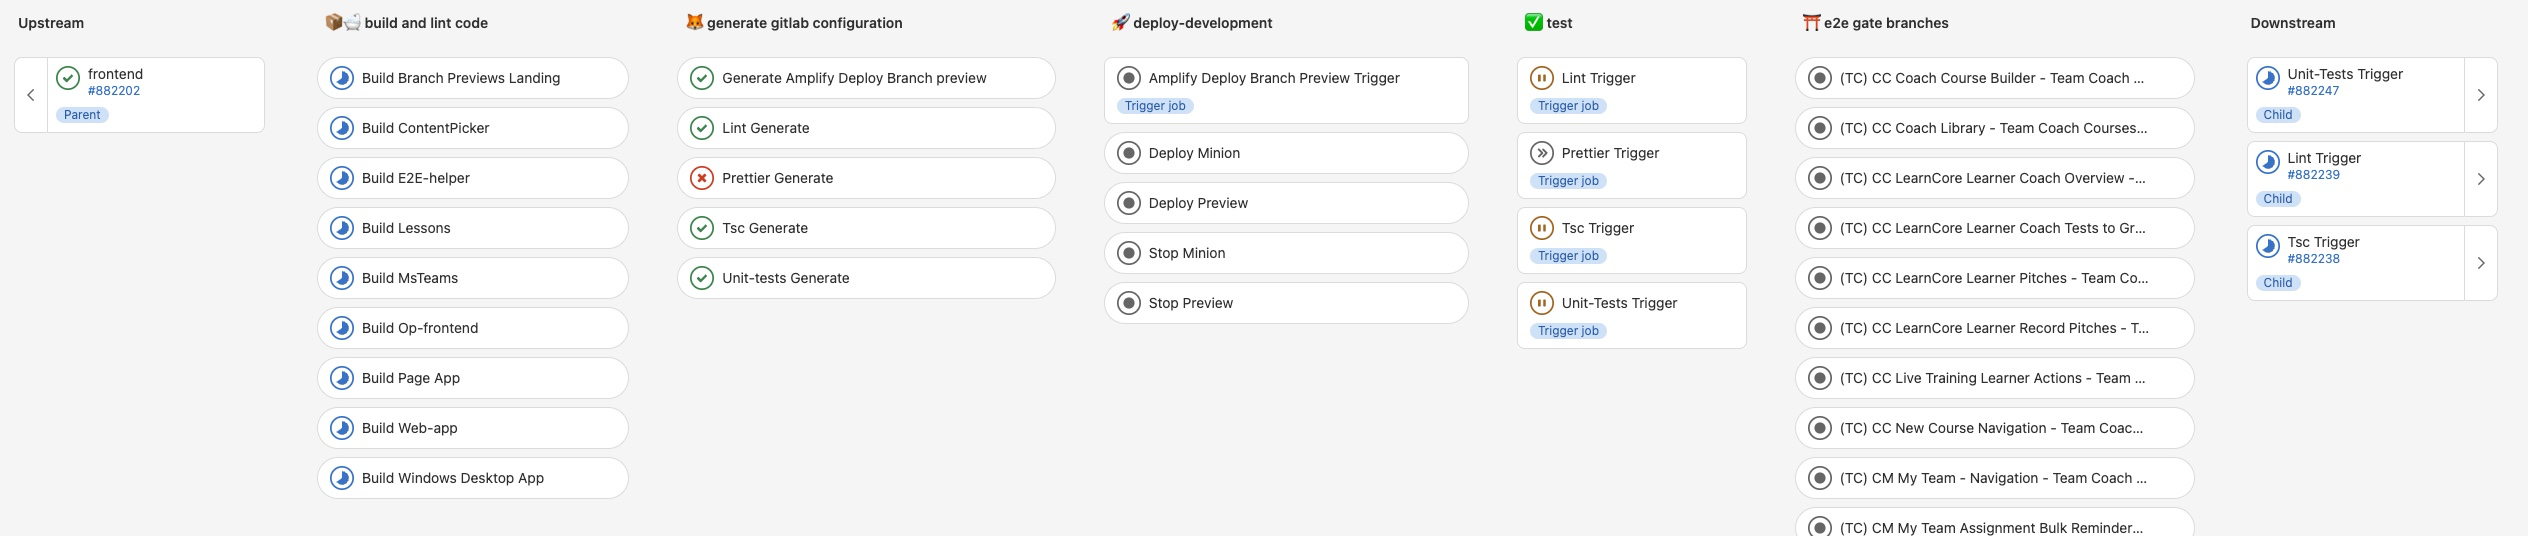
\includegraphics[width=15cm]{pipeline}
    \caption{Screenshot of current pipeline within Showpad}
\end{figure}

\section{Metric baseline}
\subsection{Build times}
If a developer wants to test his changes locally, he needs to build the entire Showpad web application. This takes on average 4 minutes and 11 seconds. Which can be frustrating to wait four minutes to just spin up the application.

\subsection{CI/CD pipeline runtime}
In the current CI/CD it sometimes takes hours to just run through the pipeline, this is mainly caused by the end-to-end tests. The pipeline without the end-to-end tests takes on average 35 minutes and 29 seconds which on its own is not that bad. The pipeline is constantly being improved so the time waiting on the pipeline is still getting better.

\subsection{Cycle Time}
The biggest problem in the cycle time in the monorepo structure is the dependability of teams on each other. They always have to wait for their code to be deployed to production, which currently happens about twice a day. A simplified version of the current process to get code into production is shown in figure 4.2.

\begin{figure}[!h]
    \centering
    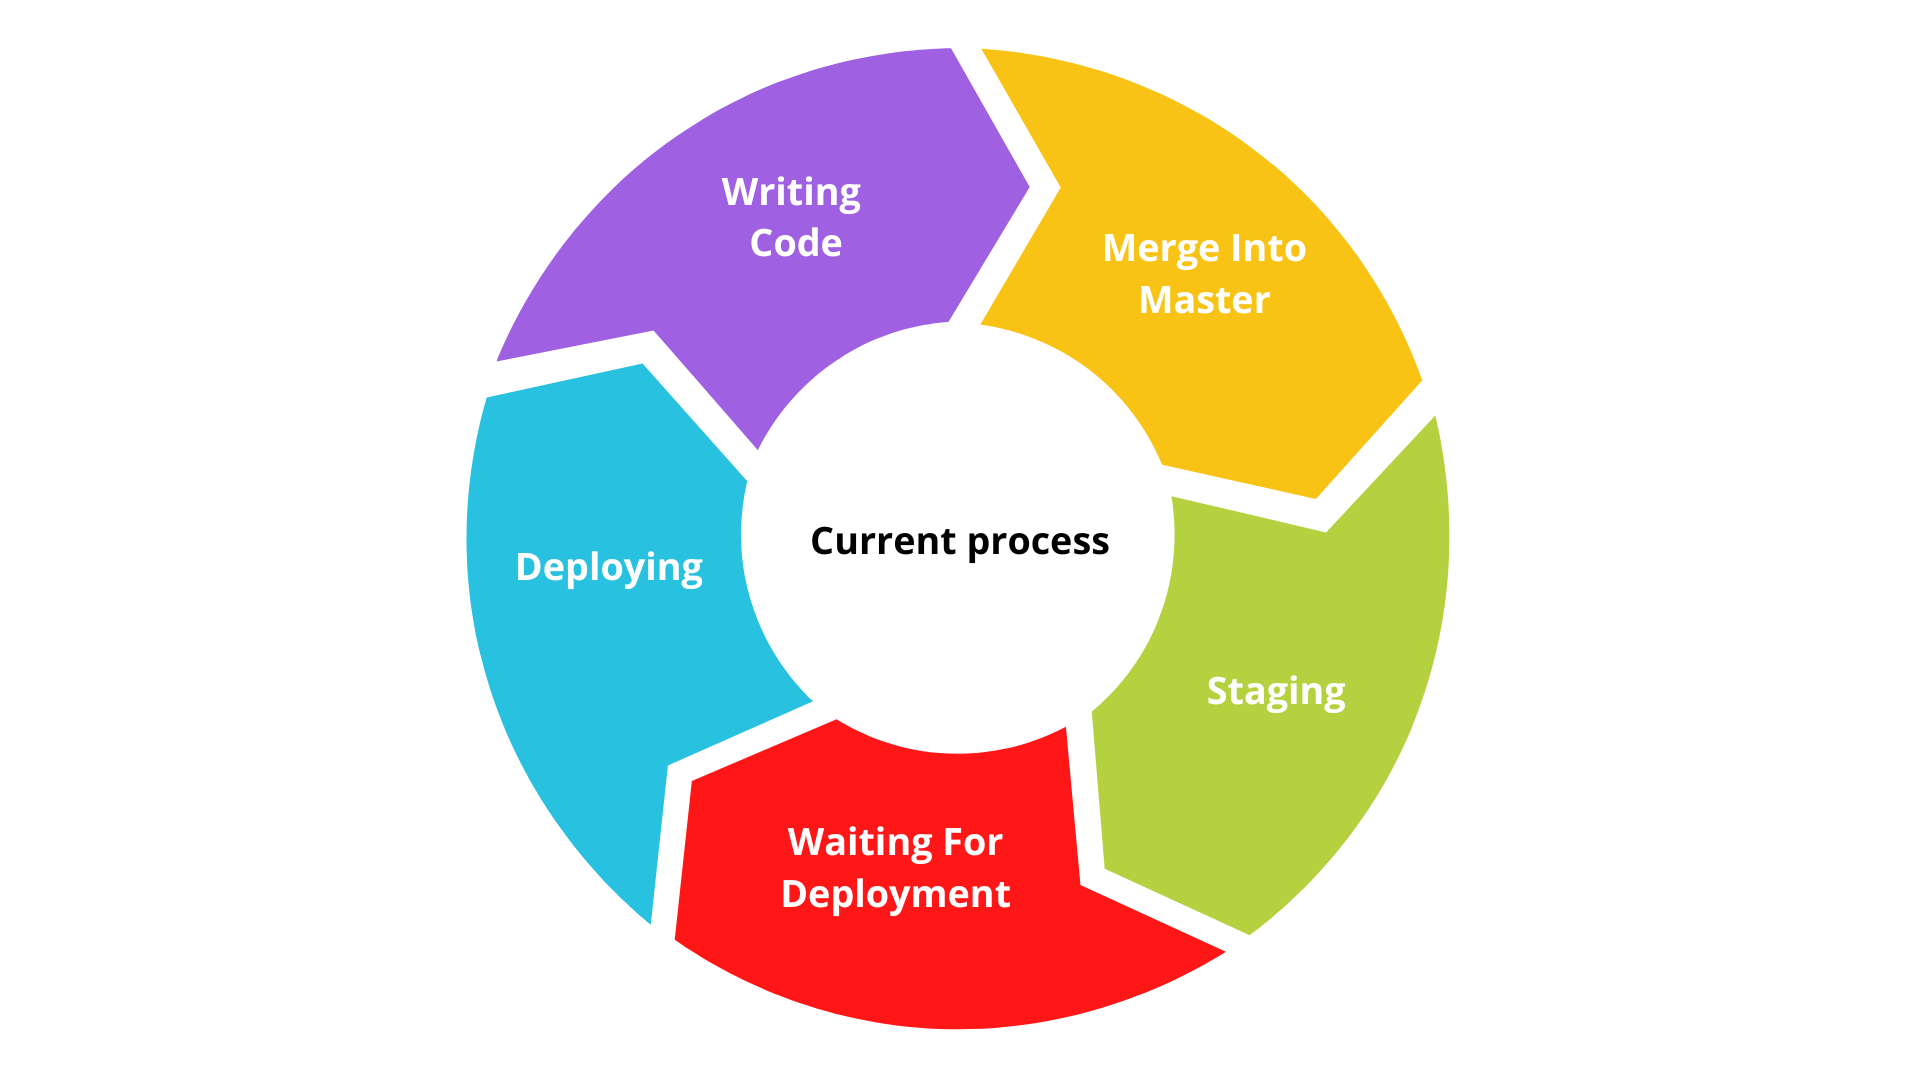
\includegraphics[width=12cm]{current-cycle}
    \caption{Simplified current process for getting code into production}
\end{figure}
